% Created by tikzDevice version 0.11 on 2018-08-26 21:55:08
% !TEX encoding = UTF-8 Unicode
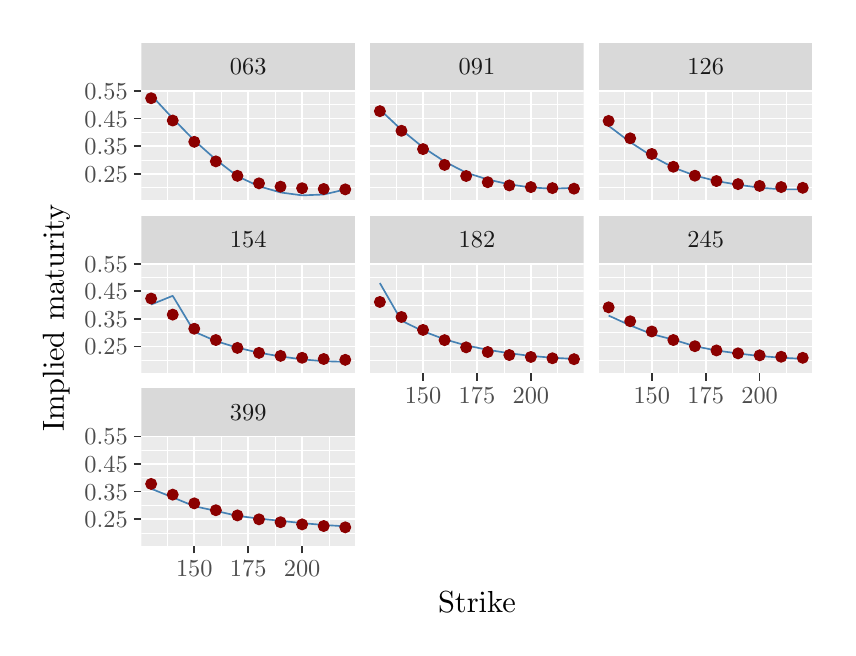
\begin{tikzpicture}[x=1pt,y=1pt]
\definecolor{fillColor}{RGB}{255,255,255}
\path[use as bounding box,fill=fillColor,fill opacity=0.00] (0,0) rectangle (289.08,216.81);
\begin{scope}
\path[clip] (  0.00,  0.00) rectangle (289.08,216.81);
\definecolor{drawColor}{RGB}{255,255,255}
\definecolor{fillColor}{RGB}{255,255,255}

\path[draw=drawColor,line width= 0.6pt,line join=round,line cap=round,fill=fillColor] (  0.00,  0.00) rectangle (289.08,216.81);
\end{scope}
\begin{scope}
\path[clip] ( 41.11,154.40) rectangle (118.27,194.25);
\definecolor{fillColor}{gray}{0.92}

\path[fill=fillColor] ( 41.11,154.40) rectangle (118.27,194.25);
\definecolor{drawColor}{RGB}{255,255,255}

\path[draw=drawColor,line width= 0.3pt,line join=round] ( 41.11,158.99) --
	(118.27,158.99);

\path[draw=drawColor,line width= 0.3pt,line join=round] ( 41.11,168.97) --
	(118.27,168.97);

\path[draw=drawColor,line width= 0.3pt,line join=round] ( 41.11,178.95) --
	(118.27,178.95);

\path[draw=drawColor,line width= 0.3pt,line join=round] ( 41.11,188.93) --
	(118.27,188.93);

\path[draw=drawColor,line width= 0.3pt,line join=round] ( 50.46,154.40) --
	( 50.46,194.25);

\path[draw=drawColor,line width= 0.3pt,line join=round] ( 69.95,154.40) --
	( 69.95,194.25);

\path[draw=drawColor,line width= 0.3pt,line join=round] ( 89.43,154.40) --
	( 89.43,194.25);

\path[draw=drawColor,line width= 0.3pt,line join=round] (108.91,154.40) --
	(108.91,194.25);

\path[draw=drawColor,line width= 0.6pt,line join=round] ( 41.11,163.98) --
	(118.27,163.98);

\path[draw=drawColor,line width= 0.6pt,line join=round] ( 41.11,173.96) --
	(118.27,173.96);

\path[draw=drawColor,line width= 0.6pt,line join=round] ( 41.11,183.94) --
	(118.27,183.94);

\path[draw=drawColor,line width= 0.6pt,line join=round] ( 41.11,193.92) --
	(118.27,193.92);

\path[draw=drawColor,line width= 0.6pt,line join=round] ( 60.20,154.40) --
	( 60.20,194.25);

\path[draw=drawColor,line width= 0.6pt,line join=round] ( 79.69,154.40) --
	( 79.69,194.25);

\path[draw=drawColor,line width= 0.6pt,line join=round] ( 99.17,154.40) --
	( 99.17,194.25);
\definecolor{drawColor}{RGB}{70,130,180}

\path[draw=drawColor,line width= 0.6pt,line join=round] ( 44.62,192.44) --
	( 52.41,184.05) --
	( 60.20,176.06) --
	( 68.00,169.13) --
	( 75.79,163.12) --
	( 83.59,159.50) --
	( 91.38,157.26) --
	( 99.17,156.21) --
	(106.97,156.52) --
	(114.76,158.35);
\definecolor{drawColor}{RGB}{139,0,0}
\definecolor{fillColor}{RGB}{139,0,0}

\path[draw=drawColor,line width= 0.4pt,line join=round,line cap=round,fill=fillColor] ( 44.62,191.32) circle (  1.96);

\path[draw=drawColor,line width= 0.4pt,line join=round,line cap=round,fill=fillColor] ( 52.41,183.25) circle (  1.96);

\path[draw=drawColor,line width= 0.4pt,line join=round,line cap=round,fill=fillColor] ( 60.20,175.56) circle (  1.96);

\path[draw=drawColor,line width= 0.4pt,line join=round,line cap=round,fill=fillColor] ( 68.00,168.49) circle (  1.96);

\path[draw=drawColor,line width= 0.4pt,line join=round,line cap=round,fill=fillColor] ( 75.79,163.27) circle (  1.96);

\path[draw=drawColor,line width= 0.4pt,line join=round,line cap=round,fill=fillColor] ( 83.59,160.56) circle (  1.96);

\path[draw=drawColor,line width= 0.4pt,line join=round,line cap=round,fill=fillColor] ( 91.38,159.36) circle (  1.96);

\path[draw=drawColor,line width= 0.4pt,line join=round,line cap=round,fill=fillColor] ( 99.17,158.80) circle (  1.96);

\path[draw=drawColor,line width= 0.4pt,line join=round,line cap=round,fill=fillColor] (106.97,158.52) circle (  1.96);

\path[draw=drawColor,line width= 0.4pt,line join=round,line cap=round,fill=fillColor] (114.76,158.38) circle (  1.96);
\end{scope}
\begin{scope}
\path[clip] ( 41.11, 91.99) rectangle (118.27,131.84);
\definecolor{fillColor}{gray}{0.92}

\path[fill=fillColor] ( 41.11, 91.99) rectangle (118.27,131.84);
\definecolor{drawColor}{RGB}{255,255,255}

\path[draw=drawColor,line width= 0.3pt,line join=round] ( 41.11, 96.59) --
	(118.27, 96.59);

\path[draw=drawColor,line width= 0.3pt,line join=round] ( 41.11,106.57) --
	(118.27,106.57);

\path[draw=drawColor,line width= 0.3pt,line join=round] ( 41.11,116.55) --
	(118.27,116.55);

\path[draw=drawColor,line width= 0.3pt,line join=round] ( 41.11,126.52) --
	(118.27,126.52);

\path[draw=drawColor,line width= 0.3pt,line join=round] ( 50.46, 91.99) --
	( 50.46,131.84);

\path[draw=drawColor,line width= 0.3pt,line join=round] ( 69.95, 91.99) --
	( 69.95,131.84);

\path[draw=drawColor,line width= 0.3pt,line join=round] ( 89.43, 91.99) --
	( 89.43,131.84);

\path[draw=drawColor,line width= 0.3pt,line join=round] (108.91, 91.99) --
	(108.91,131.84);

\path[draw=drawColor,line width= 0.6pt,line join=round] ( 41.11,101.58) --
	(118.27,101.58);

\path[draw=drawColor,line width= 0.6pt,line join=round] ( 41.11,111.56) --
	(118.27,111.56);

\path[draw=drawColor,line width= 0.6pt,line join=round] ( 41.11,121.54) --
	(118.27,121.54);

\path[draw=drawColor,line width= 0.6pt,line join=round] ( 41.11,131.51) --
	(118.27,131.51);

\path[draw=drawColor,line width= 0.6pt,line join=round] ( 60.20, 91.99) --
	( 60.20,131.84);

\path[draw=drawColor,line width= 0.6pt,line join=round] ( 79.69, 91.99) --
	( 79.69,131.84);

\path[draw=drawColor,line width= 0.6pt,line join=round] ( 99.17, 91.99) --
	( 99.17,131.84);
\definecolor{drawColor}{RGB}{70,130,180}

\path[draw=drawColor,line width= 0.6pt,line join=round] ( 44.62,116.76) --
	( 52.41,119.91) --
	( 60.20,106.96) --
	( 68.00,103.57) --
	( 75.79,101.17) --
	( 83.59, 99.36) --
	( 91.38, 98.01) --
	( 99.17, 96.95) --
	(106.97, 96.29) --
	(114.76, 96.06);
\definecolor{drawColor}{RGB}{139,0,0}
\definecolor{fillColor}{RGB}{139,0,0}

\path[draw=drawColor,line width= 0.4pt,line join=round,line cap=round,fill=fillColor] ( 44.62,118.93) circle (  1.96);

\path[draw=drawColor,line width= 0.4pt,line join=round,line cap=round,fill=fillColor] ( 52.41,113.12) circle (  1.96);

\path[draw=drawColor,line width= 0.4pt,line join=round,line cap=round,fill=fillColor] ( 60.20,108.02) circle (  1.96);

\path[draw=drawColor,line width= 0.4pt,line join=round,line cap=round,fill=fillColor] ( 68.00,103.94) circle (  1.96);

\path[draw=drawColor,line width= 0.4pt,line join=round,line cap=round,fill=fillColor] ( 75.79,101.09) circle (  1.96);

\path[draw=drawColor,line width= 0.4pt,line join=round,line cap=round,fill=fillColor] ( 83.59, 99.30) circle (  1.96);

\path[draw=drawColor,line width= 0.4pt,line join=round,line cap=round,fill=fillColor] ( 91.38, 98.21) circle (  1.96);

\path[draw=drawColor,line width= 0.4pt,line join=round,line cap=round,fill=fillColor] ( 99.17, 97.52) circle (  1.96);

\path[draw=drawColor,line width= 0.4pt,line join=round,line cap=round,fill=fillColor] (106.97, 97.08) circle (  1.96);

\path[draw=drawColor,line width= 0.4pt,line join=round,line cap=round,fill=fillColor] (114.76, 96.78) circle (  1.96);
\end{scope}
\begin{scope}
\path[clip] ( 41.11, 29.59) rectangle (118.27, 69.43);
\definecolor{fillColor}{gray}{0.92}

\path[fill=fillColor] ( 41.11, 29.59) rectangle (118.27, 69.43);
\definecolor{drawColor}{RGB}{255,255,255}

\path[draw=drawColor,line width= 0.3pt,line join=round] ( 41.11, 34.18) --
	(118.27, 34.18);

\path[draw=drawColor,line width= 0.3pt,line join=round] ( 41.11, 44.16) --
	(118.27, 44.16);

\path[draw=drawColor,line width= 0.3pt,line join=round] ( 41.11, 54.14) --
	(118.27, 54.14);

\path[draw=drawColor,line width= 0.3pt,line join=round] ( 41.11, 64.12) --
	(118.27, 64.12);

\path[draw=drawColor,line width= 0.3pt,line join=round] ( 50.46, 29.59) --
	( 50.46, 69.43);

\path[draw=drawColor,line width= 0.3pt,line join=round] ( 69.95, 29.59) --
	( 69.95, 69.43);

\path[draw=drawColor,line width= 0.3pt,line join=round] ( 89.43, 29.59) --
	( 89.43, 69.43);

\path[draw=drawColor,line width= 0.3pt,line join=round] (108.91, 29.59) --
	(108.91, 69.43);

\path[draw=drawColor,line width= 0.6pt,line join=round] ( 41.11, 39.17) --
	(118.27, 39.17);

\path[draw=drawColor,line width= 0.6pt,line join=round] ( 41.11, 49.15) --
	(118.27, 49.15);

\path[draw=drawColor,line width= 0.6pt,line join=round] ( 41.11, 59.13) --
	(118.27, 59.13);

\path[draw=drawColor,line width= 0.6pt,line join=round] ( 41.11, 69.11) --
	(118.27, 69.11);

\path[draw=drawColor,line width= 0.6pt,line join=round] ( 60.20, 29.59) --
	( 60.20, 69.43);

\path[draw=drawColor,line width= 0.6pt,line join=round] ( 79.69, 29.59) --
	( 79.69, 69.43);

\path[draw=drawColor,line width= 0.6pt,line join=round] ( 99.17, 29.59) --
	( 99.17, 69.43);
\definecolor{drawColor}{RGB}{70,130,180}

\path[draw=drawColor,line width= 0.6pt,line join=round] ( 44.62, 50.20) --
	( 52.41, 47.09) --
	( 60.20, 43.89) --
	( 68.00, 42.20) --
	( 75.79, 40.40) --
	( 83.59, 39.42) --
	( 91.38, 38.61) --
	( 99.17, 37.78) --
	(106.97, 37.11) --
	(114.76, 36.62);
\definecolor{drawColor}{RGB}{139,0,0}
\definecolor{fillColor}{RGB}{139,0,0}

\path[draw=drawColor,line width= 0.4pt,line join=round,line cap=round,fill=fillColor] ( 44.62, 51.94) circle (  1.96);

\path[draw=drawColor,line width= 0.4pt,line join=round,line cap=round,fill=fillColor] ( 52.41, 48.07) circle (  1.96);

\path[draw=drawColor,line width= 0.4pt,line join=round,line cap=round,fill=fillColor] ( 60.20, 44.92) circle (  1.96);

\path[draw=drawColor,line width= 0.4pt,line join=round,line cap=round,fill=fillColor] ( 68.00, 42.44) circle (  1.96);

\path[draw=drawColor,line width= 0.4pt,line join=round,line cap=round,fill=fillColor] ( 75.79, 40.56) circle (  1.96);

\path[draw=drawColor,line width= 0.4pt,line join=round,line cap=round,fill=fillColor] ( 83.59, 39.15) circle (  1.96);

\path[draw=drawColor,line width= 0.4pt,line join=round,line cap=round,fill=fillColor] ( 91.38, 38.11) circle (  1.96);

\path[draw=drawColor,line width= 0.4pt,line join=round,line cap=round,fill=fillColor] ( 99.17, 37.32) circle (  1.96);

\path[draw=drawColor,line width= 0.4pt,line join=round,line cap=round,fill=fillColor] (106.97, 36.73) circle (  1.96);

\path[draw=drawColor,line width= 0.4pt,line join=round,line cap=round,fill=fillColor] (114.76, 36.26) circle (  1.96);
\end{scope}
\begin{scope}
\path[clip] (123.77,154.40) rectangle (200.92,194.25);
\definecolor{fillColor}{gray}{0.92}

\path[fill=fillColor] (123.77,154.40) rectangle (200.92,194.25);
\definecolor{drawColor}{RGB}{255,255,255}

\path[draw=drawColor,line width= 0.3pt,line join=round] (123.77,158.99) --
	(200.92,158.99);

\path[draw=drawColor,line width= 0.3pt,line join=round] (123.77,168.97) --
	(200.92,168.97);

\path[draw=drawColor,line width= 0.3pt,line join=round] (123.77,178.95) --
	(200.92,178.95);

\path[draw=drawColor,line width= 0.3pt,line join=round] (123.77,188.93) --
	(200.92,188.93);

\path[draw=drawColor,line width= 0.3pt,line join=round] (133.12,154.40) --
	(133.12,194.25);

\path[draw=drawColor,line width= 0.3pt,line join=round] (152.60,154.40) --
	(152.60,194.25);

\path[draw=drawColor,line width= 0.3pt,line join=round] (172.09,154.40) --
	(172.09,194.25);

\path[draw=drawColor,line width= 0.3pt,line join=round] (191.57,154.40) --
	(191.57,194.25);

\path[draw=drawColor,line width= 0.6pt,line join=round] (123.77,163.98) --
	(200.92,163.98);

\path[draw=drawColor,line width= 0.6pt,line join=round] (123.77,173.96) --
	(200.92,173.96);

\path[draw=drawColor,line width= 0.6pt,line join=round] (123.77,183.94) --
	(200.92,183.94);

\path[draw=drawColor,line width= 0.6pt,line join=round] (123.77,193.92) --
	(200.92,193.92);

\path[draw=drawColor,line width= 0.6pt,line join=round] (142.86,154.40) --
	(142.86,194.25);

\path[draw=drawColor,line width= 0.6pt,line join=round] (162.35,154.40) --
	(162.35,194.25);

\path[draw=drawColor,line width= 0.6pt,line join=round] (181.83,154.40) --
	(181.83,194.25);
\definecolor{drawColor}{RGB}{70,130,180}

\path[draw=drawColor,line width= 0.6pt,line join=round] (127.27,187.21) --
	(135.07,179.91) --
	(142.86,173.56) --
	(150.65,168.42) --
	(158.45,164.40) --
	(166.24,161.96) --
	(174.04,160.18) --
	(181.83,159.07) --
	(189.62,158.62) --
	(197.42,158.94);
\definecolor{drawColor}{RGB}{139,0,0}
\definecolor{fillColor}{RGB}{139,0,0}

\path[draw=drawColor,line width= 0.4pt,line join=round,line cap=round,fill=fillColor] (127.27,186.64) circle (  1.96);

\path[draw=drawColor,line width= 0.4pt,line join=round,line cap=round,fill=fillColor] (135.07,179.55) circle (  1.96);

\path[draw=drawColor,line width= 0.4pt,line join=round,line cap=round,fill=fillColor] (142.86,172.93) circle (  1.96);

\path[draw=drawColor,line width= 0.4pt,line join=round,line cap=round,fill=fillColor] (150.65,167.22) circle (  1.96);

\path[draw=drawColor,line width= 0.4pt,line join=round,line cap=round,fill=fillColor] (158.45,163.21) circle (  1.96);

\path[draw=drawColor,line width= 0.4pt,line join=round,line cap=round,fill=fillColor] (166.24,160.97) circle (  1.96);

\path[draw=drawColor,line width= 0.4pt,line join=round,line cap=round,fill=fillColor] (174.04,159.81) circle (  1.96);

\path[draw=drawColor,line width= 0.4pt,line join=round,line cap=round,fill=fillColor] (181.83,159.20) circle (  1.96);

\path[draw=drawColor,line width= 0.4pt,line join=round,line cap=round,fill=fillColor] (189.62,158.84) circle (  1.96);

\path[draw=drawColor,line width= 0.4pt,line join=round,line cap=round,fill=fillColor] (197.42,158.63) circle (  1.96);
\end{scope}
\begin{scope}
\path[clip] (123.77, 91.99) rectangle (200.92,131.84);
\definecolor{fillColor}{gray}{0.92}

\path[fill=fillColor] (123.77, 91.99) rectangle (200.92,131.84);
\definecolor{drawColor}{RGB}{255,255,255}

\path[draw=drawColor,line width= 0.3pt,line join=round] (123.77, 96.59) --
	(200.92, 96.59);

\path[draw=drawColor,line width= 0.3pt,line join=round] (123.77,106.57) --
	(200.92,106.57);

\path[draw=drawColor,line width= 0.3pt,line join=round] (123.77,116.55) --
	(200.92,116.55);

\path[draw=drawColor,line width= 0.3pt,line join=round] (123.77,126.52) --
	(200.92,126.52);

\path[draw=drawColor,line width= 0.3pt,line join=round] (133.12, 91.99) --
	(133.12,131.84);

\path[draw=drawColor,line width= 0.3pt,line join=round] (152.60, 91.99) --
	(152.60,131.84);

\path[draw=drawColor,line width= 0.3pt,line join=round] (172.09, 91.99) --
	(172.09,131.84);

\path[draw=drawColor,line width= 0.3pt,line join=round] (191.57, 91.99) --
	(191.57,131.84);

\path[draw=drawColor,line width= 0.6pt,line join=round] (123.77,101.58) --
	(200.92,101.58);

\path[draw=drawColor,line width= 0.6pt,line join=round] (123.77,111.56) --
	(200.92,111.56);

\path[draw=drawColor,line width= 0.6pt,line join=round] (123.77,121.54) --
	(200.92,121.54);

\path[draw=drawColor,line width= 0.6pt,line join=round] (123.77,131.51) --
	(200.92,131.51);

\path[draw=drawColor,line width= 0.6pt,line join=round] (142.86, 91.99) --
	(142.86,131.84);

\path[draw=drawColor,line width= 0.6pt,line join=round] (162.35, 91.99) --
	(162.35,131.84);

\path[draw=drawColor,line width= 0.6pt,line join=round] (181.83, 91.99) --
	(181.83,131.84);
\definecolor{drawColor}{RGB}{70,130,180}

\path[draw=drawColor,line width= 0.6pt,line join=round] (127.27,124.51) --
	(135.07,110.93) --
	(142.86,107.13) --
	(150.65,104.20) --
	(158.45,101.98) --
	(166.24,100.40) --
	(174.04, 99.17) --
	(181.83, 98.18) --
	(189.62, 97.55) --
	(197.42, 97.12);
\definecolor{drawColor}{RGB}{139,0,0}
\definecolor{fillColor}{RGB}{139,0,0}

\path[draw=drawColor,line width= 0.4pt,line join=round,line cap=round,fill=fillColor] (127.27,117.69) circle (  1.96);

\path[draw=drawColor,line width= 0.4pt,line join=round,line cap=round,fill=fillColor] (135.07,112.26) circle (  1.96);

\path[draw=drawColor,line width= 0.4pt,line join=round,line cap=round,fill=fillColor] (142.86,107.59) circle (  1.96);

\path[draw=drawColor,line width= 0.4pt,line join=round,line cap=round,fill=fillColor] (150.65,103.90) circle (  1.96);

\path[draw=drawColor,line width= 0.4pt,line join=round,line cap=round,fill=fillColor] (158.45,101.30) circle (  1.96);

\path[draw=drawColor,line width= 0.4pt,line join=round,line cap=round,fill=fillColor] (166.24, 99.61) circle (  1.96);

\path[draw=drawColor,line width= 0.4pt,line join=round,line cap=round,fill=fillColor] (174.04, 98.52) circle (  1.96);

\path[draw=drawColor,line width= 0.4pt,line join=round,line cap=round,fill=fillColor] (181.83, 97.82) circle (  1.96);

\path[draw=drawColor,line width= 0.4pt,line join=round,line cap=round,fill=fillColor] (189.62, 97.35) circle (  1.96);

\path[draw=drawColor,line width= 0.4pt,line join=round,line cap=round,fill=fillColor] (197.42, 97.02) circle (  1.96);
\end{scope}
\begin{scope}
\path[clip] (206.42,154.40) rectangle (283.58,194.25);
\definecolor{fillColor}{gray}{0.92}

\path[fill=fillColor] (206.42,154.40) rectangle (283.58,194.25);
\definecolor{drawColor}{RGB}{255,255,255}

\path[draw=drawColor,line width= 0.3pt,line join=round] (206.42,158.99) --
	(283.58,158.99);

\path[draw=drawColor,line width= 0.3pt,line join=round] (206.42,168.97) --
	(283.58,168.97);

\path[draw=drawColor,line width= 0.3pt,line join=round] (206.42,178.95) --
	(283.58,178.95);

\path[draw=drawColor,line width= 0.3pt,line join=round] (206.42,188.93) --
	(283.58,188.93);

\path[draw=drawColor,line width= 0.3pt,line join=round] (215.78,154.40) --
	(215.78,194.25);

\path[draw=drawColor,line width= 0.3pt,line join=round] (235.26,154.40) --
	(235.26,194.25);

\path[draw=drawColor,line width= 0.3pt,line join=round] (254.74,154.40) --
	(254.74,194.25);

\path[draw=drawColor,line width= 0.3pt,line join=round] (274.23,154.40) --
	(274.23,194.25);

\path[draw=drawColor,line width= 0.6pt,line join=round] (206.42,163.98) --
	(283.58,163.98);

\path[draw=drawColor,line width= 0.6pt,line join=round] (206.42,173.96) --
	(283.58,173.96);

\path[draw=drawColor,line width= 0.6pt,line join=round] (206.42,183.94) --
	(283.58,183.94);

\path[draw=drawColor,line width= 0.6pt,line join=round] (206.42,193.92) --
	(283.58,193.92);

\path[draw=drawColor,line width= 0.6pt,line join=round] (225.52,154.40) --
	(225.52,194.25);

\path[draw=drawColor,line width= 0.6pt,line join=round] (245.00,154.40) --
	(245.00,194.25);

\path[draw=drawColor,line width= 0.6pt,line join=round] (264.49,154.40) --
	(264.49,194.25);
\definecolor{drawColor}{RGB}{70,130,180}

\path[draw=drawColor,line width= 0.6pt,line join=round] (209.93,181.34) --
	(217.72,175.45) --
	(225.52,170.41) --
	(233.31,166.28) --
	(241.10,163.37) --
	(248.90,161.38) --
	(256.69,160.05) --
	(264.49,158.99) --
	(272.28,158.40) --
	(280.07,158.35);
\definecolor{drawColor}{RGB}{139,0,0}
\definecolor{fillColor}{RGB}{139,0,0}

\path[draw=drawColor,line width= 0.4pt,line join=round,line cap=round,fill=fillColor] (209.93,183.11) circle (  1.96);

\path[draw=drawColor,line width= 0.4pt,line join=round,line cap=round,fill=fillColor] (217.72,176.83) circle (  1.96);

\path[draw=drawColor,line width= 0.4pt,line join=round,line cap=round,fill=fillColor] (225.52,171.17) circle (  1.96);

\path[draw=drawColor,line width= 0.4pt,line join=round,line cap=round,fill=fillColor] (233.31,166.54) circle (  1.96);

\path[draw=drawColor,line width= 0.4pt,line join=round,line cap=round,fill=fillColor] (241.10,163.32) circle (  1.96);

\path[draw=drawColor,line width= 0.4pt,line join=round,line cap=round,fill=fillColor] (248.90,161.39) circle (  1.96);

\path[draw=drawColor,line width= 0.4pt,line join=round,line cap=round,fill=fillColor] (256.69,160.28) circle (  1.96);

\path[draw=drawColor,line width= 0.4pt,line join=round,line cap=round,fill=fillColor] (264.49,159.62) circle (  1.96);

\path[draw=drawColor,line width= 0.4pt,line join=round,line cap=round,fill=fillColor] (272.28,159.21) circle (  1.96);

\path[draw=drawColor,line width= 0.4pt,line join=round,line cap=round,fill=fillColor] (280.07,158.94) circle (  1.96);
\end{scope}
\begin{scope}
\path[clip] (206.42, 91.99) rectangle (283.58,131.84);
\definecolor{fillColor}{gray}{0.92}

\path[fill=fillColor] (206.42, 91.99) rectangle (283.58,131.84);
\definecolor{drawColor}{RGB}{255,255,255}

\path[draw=drawColor,line width= 0.3pt,line join=round] (206.42, 96.59) --
	(283.58, 96.59);

\path[draw=drawColor,line width= 0.3pt,line join=round] (206.42,106.57) --
	(283.58,106.57);

\path[draw=drawColor,line width= 0.3pt,line join=round] (206.42,116.55) --
	(283.58,116.55);

\path[draw=drawColor,line width= 0.3pt,line join=round] (206.42,126.52) --
	(283.58,126.52);

\path[draw=drawColor,line width= 0.3pt,line join=round] (215.78, 91.99) --
	(215.78,131.84);

\path[draw=drawColor,line width= 0.3pt,line join=round] (235.26, 91.99) --
	(235.26,131.84);

\path[draw=drawColor,line width= 0.3pt,line join=round] (254.74, 91.99) --
	(254.74,131.84);

\path[draw=drawColor,line width= 0.3pt,line join=round] (274.23, 91.99) --
	(274.23,131.84);

\path[draw=drawColor,line width= 0.6pt,line join=round] (206.42,101.58) --
	(283.58,101.58);

\path[draw=drawColor,line width= 0.6pt,line join=round] (206.42,111.56) --
	(283.58,111.56);

\path[draw=drawColor,line width= 0.6pt,line join=round] (206.42,121.54) --
	(283.58,121.54);

\path[draw=drawColor,line width= 0.6pt,line join=round] (206.42,131.51) --
	(283.58,131.51);

\path[draw=drawColor,line width= 0.6pt,line join=round] (225.52, 91.99) --
	(225.52,131.84);

\path[draw=drawColor,line width= 0.6pt,line join=round] (245.00, 91.99) --
	(245.00,131.84);

\path[draw=drawColor,line width= 0.6pt,line join=round] (264.49, 91.99) --
	(264.49,131.84);
\definecolor{drawColor}{RGB}{70,130,180}

\path[draw=drawColor,line width= 0.6pt,line join=round] (209.93,112.77) --
	(217.72,109.24) --
	(225.52,106.08) --
	(233.31,104.08) --
	(241.10,101.69) --
	(248.90,100.16) --
	(256.69, 99.08) --
	(264.49, 98.16) --
	(272.28, 97.55) --
	(280.07, 97.14);
\definecolor{drawColor}{RGB}{139,0,0}
\definecolor{fillColor}{RGB}{139,0,0}

\path[draw=drawColor,line width= 0.4pt,line join=round,line cap=round,fill=fillColor] (209.93,115.75) circle (  1.96);

\path[draw=drawColor,line width= 0.4pt,line join=round,line cap=round,fill=fillColor] (217.72,110.73) circle (  1.96);

\path[draw=drawColor,line width= 0.4pt,line join=round,line cap=round,fill=fillColor] (225.52,107.03) circle (  1.96);

\path[draw=drawColor,line width= 0.4pt,line join=round,line cap=round,fill=fillColor] (233.31,103.94) circle (  1.96);

\path[draw=drawColor,line width= 0.4pt,line join=round,line cap=round,fill=fillColor] (241.10,101.71) circle (  1.96);

\path[draw=drawColor,line width= 0.4pt,line join=round,line cap=round,fill=fillColor] (248.90,100.18) circle (  1.96);

\path[draw=drawColor,line width= 0.4pt,line join=round,line cap=round,fill=fillColor] (256.69, 99.13) circle (  1.96);

\path[draw=drawColor,line width= 0.4pt,line join=round,line cap=round,fill=fillColor] (264.49, 98.40) circle (  1.96);

\path[draw=drawColor,line width= 0.4pt,line join=round,line cap=round,fill=fillColor] (272.28, 97.89) circle (  1.96);

\path[draw=drawColor,line width= 0.4pt,line join=round,line cap=round,fill=fillColor] (280.07, 97.51) circle (  1.96);
\end{scope}
\begin{scope}
\path[clip] ( 41.11, 69.43) rectangle (118.27, 86.49);
\definecolor{fillColor}{gray}{0.85}

\path[fill=fillColor] ( 41.11, 69.43) rectangle (118.27, 86.49);
\definecolor{drawColor}{gray}{0.10}

\node[text=drawColor,anchor=base,inner sep=0pt, outer sep=0pt, scale=  0.88] at ( 79.69, 74.93) {399};
\end{scope}
\begin{scope}
\path[clip] ( 41.11,131.84) rectangle (118.27,148.90);
\definecolor{fillColor}{gray}{0.85}

\path[fill=fillColor] ( 41.11,131.84) rectangle (118.27,148.90);
\definecolor{drawColor}{gray}{0.10}

\node[text=drawColor,anchor=base,inner sep=0pt, outer sep=0pt, scale=  0.88] at ( 79.69,137.34) {154};
\end{scope}
\begin{scope}
\path[clip] (123.77,131.84) rectangle (200.92,148.90);
\definecolor{fillColor}{gray}{0.85}

\path[fill=fillColor] (123.77,131.84) rectangle (200.92,148.90);
\definecolor{drawColor}{gray}{0.10}

\node[text=drawColor,anchor=base,inner sep=0pt, outer sep=0pt, scale=  0.88] at (162.35,137.34) {182};
\end{scope}
\begin{scope}
\path[clip] (206.42,131.84) rectangle (283.58,148.90);
\definecolor{fillColor}{gray}{0.85}

\path[fill=fillColor] (206.42,131.84) rectangle (283.58,148.90);
\definecolor{drawColor}{gray}{0.10}

\node[text=drawColor,anchor=base,inner sep=0pt, outer sep=0pt, scale=  0.88] at (245.00,137.34) {245};
\end{scope}
\begin{scope}
\path[clip] ( 41.11,194.25) rectangle (118.27,211.31);
\definecolor{fillColor}{gray}{0.85}

\path[fill=fillColor] ( 41.11,194.25) rectangle (118.27,211.31);
\definecolor{drawColor}{gray}{0.10}

\node[text=drawColor,anchor=base,inner sep=0pt, outer sep=0pt, scale=  0.88] at ( 79.69,199.75) {063};
\end{scope}
\begin{scope}
\path[clip] (123.77,194.25) rectangle (200.92,211.31);
\definecolor{fillColor}{gray}{0.85}

\path[fill=fillColor] (123.77,194.25) rectangle (200.92,211.31);
\definecolor{drawColor}{gray}{0.10}

\node[text=drawColor,anchor=base,inner sep=0pt, outer sep=0pt, scale=  0.88] at (162.35,199.75) {091};
\end{scope}
\begin{scope}
\path[clip] (206.42,194.25) rectangle (283.58,211.31);
\definecolor{fillColor}{gray}{0.85}

\path[fill=fillColor] (206.42,194.25) rectangle (283.58,211.31);
\definecolor{drawColor}{gray}{0.10}

\node[text=drawColor,anchor=base,inner sep=0pt, outer sep=0pt, scale=  0.88] at (245.00,199.75) {126};
\end{scope}
\begin{scope}
\path[clip] (  0.00,  0.00) rectangle (289.08,216.81);
\definecolor{drawColor}{gray}{0.20}

\path[draw=drawColor,line width= 0.6pt,line join=round] ( 60.20, 26.84) --
	( 60.20, 29.59);

\path[draw=drawColor,line width= 0.6pt,line join=round] ( 79.69, 26.84) --
	( 79.69, 29.59);

\path[draw=drawColor,line width= 0.6pt,line join=round] ( 99.17, 26.84) --
	( 99.17, 29.59);
\end{scope}
\begin{scope}
\path[clip] (  0.00,  0.00) rectangle (289.08,216.81);
\definecolor{drawColor}{gray}{0.30}

\node[text=drawColor,anchor=base,inner sep=0pt, outer sep=0pt, scale=  0.88] at ( 60.20, 18.58) {150};

\node[text=drawColor,anchor=base,inner sep=0pt, outer sep=0pt, scale=  0.88] at ( 79.69, 18.58) {175};

\node[text=drawColor,anchor=base,inner sep=0pt, outer sep=0pt, scale=  0.88] at ( 99.17, 18.58) {200};
\end{scope}
\begin{scope}
\path[clip] (  0.00,  0.00) rectangle (289.08,216.81);
\definecolor{drawColor}{gray}{0.20}

\path[draw=drawColor,line width= 0.6pt,line join=round] (142.86, 89.24) --
	(142.86, 91.99);

\path[draw=drawColor,line width= 0.6pt,line join=round] (162.35, 89.24) --
	(162.35, 91.99);

\path[draw=drawColor,line width= 0.6pt,line join=round] (181.83, 89.24) --
	(181.83, 91.99);
\end{scope}
\begin{scope}
\path[clip] (  0.00,  0.00) rectangle (289.08,216.81);
\definecolor{drawColor}{gray}{0.30}

\node[text=drawColor,anchor=base,inner sep=0pt, outer sep=0pt, scale=  0.88] at (142.86, 80.98) {150};

\node[text=drawColor,anchor=base,inner sep=0pt, outer sep=0pt, scale=  0.88] at (162.35, 80.98) {175};

\node[text=drawColor,anchor=base,inner sep=0pt, outer sep=0pt, scale=  0.88] at (181.83, 80.98) {200};
\end{scope}
\begin{scope}
\path[clip] (  0.00,  0.00) rectangle (289.08,216.81);
\definecolor{drawColor}{gray}{0.20}

\path[draw=drawColor,line width= 0.6pt,line join=round] (225.52, 89.24) --
	(225.52, 91.99);

\path[draw=drawColor,line width= 0.6pt,line join=round] (245.00, 89.24) --
	(245.00, 91.99);

\path[draw=drawColor,line width= 0.6pt,line join=round] (264.49, 89.24) --
	(264.49, 91.99);
\end{scope}
\begin{scope}
\path[clip] (  0.00,  0.00) rectangle (289.08,216.81);
\definecolor{drawColor}{gray}{0.30}

\node[text=drawColor,anchor=base,inner sep=0pt, outer sep=0pt, scale=  0.88] at (225.52, 80.98) {150};

\node[text=drawColor,anchor=base,inner sep=0pt, outer sep=0pt, scale=  0.88] at (245.00, 80.98) {175};

\node[text=drawColor,anchor=base,inner sep=0pt, outer sep=0pt, scale=  0.88] at (264.49, 80.98) {200};
\end{scope}
\begin{scope}
\path[clip] (  0.00,  0.00) rectangle (289.08,216.81);
\definecolor{drawColor}{gray}{0.30}

\node[text=drawColor,anchor=base east,inner sep=0pt, outer sep=0pt, scale=  0.88] at ( 36.16,160.95) {0.25};

\node[text=drawColor,anchor=base east,inner sep=0pt, outer sep=0pt, scale=  0.88] at ( 36.16,170.93) {0.35};

\node[text=drawColor,anchor=base east,inner sep=0pt, outer sep=0pt, scale=  0.88] at ( 36.16,180.91) {0.45};

\node[text=drawColor,anchor=base east,inner sep=0pt, outer sep=0pt, scale=  0.88] at ( 36.16,190.89) {0.55};
\end{scope}
\begin{scope}
\path[clip] (  0.00,  0.00) rectangle (289.08,216.81);
\definecolor{drawColor}{gray}{0.20}

\path[draw=drawColor,line width= 0.6pt,line join=round] ( 38.36,163.98) --
	( 41.11,163.98);

\path[draw=drawColor,line width= 0.6pt,line join=round] ( 38.36,173.96) --
	( 41.11,173.96);

\path[draw=drawColor,line width= 0.6pt,line join=round] ( 38.36,183.94) --
	( 41.11,183.94);

\path[draw=drawColor,line width= 0.6pt,line join=round] ( 38.36,193.92) --
	( 41.11,193.92);
\end{scope}
\begin{scope}
\path[clip] (  0.00,  0.00) rectangle (289.08,216.81);
\definecolor{drawColor}{gray}{0.30}

\node[text=drawColor,anchor=base east,inner sep=0pt, outer sep=0pt, scale=  0.88] at ( 36.16, 98.55) {0.25};

\node[text=drawColor,anchor=base east,inner sep=0pt, outer sep=0pt, scale=  0.88] at ( 36.16,108.52) {0.35};

\node[text=drawColor,anchor=base east,inner sep=0pt, outer sep=0pt, scale=  0.88] at ( 36.16,118.50) {0.45};

\node[text=drawColor,anchor=base east,inner sep=0pt, outer sep=0pt, scale=  0.88] at ( 36.16,128.48) {0.55};
\end{scope}
\begin{scope}
\path[clip] (  0.00,  0.00) rectangle (289.08,216.81);
\definecolor{drawColor}{gray}{0.20}

\path[draw=drawColor,line width= 0.6pt,line join=round] ( 38.36,101.58) --
	( 41.11,101.58);

\path[draw=drawColor,line width= 0.6pt,line join=round] ( 38.36,111.56) --
	( 41.11,111.56);

\path[draw=drawColor,line width= 0.6pt,line join=round] ( 38.36,121.54) --
	( 41.11,121.54);

\path[draw=drawColor,line width= 0.6pt,line join=round] ( 38.36,131.51) --
	( 41.11,131.51);
\end{scope}
\begin{scope}
\path[clip] (  0.00,  0.00) rectangle (289.08,216.81);
\definecolor{drawColor}{gray}{0.30}

\node[text=drawColor,anchor=base east,inner sep=0pt, outer sep=0pt, scale=  0.88] at ( 36.16, 36.14) {0.25};

\node[text=drawColor,anchor=base east,inner sep=0pt, outer sep=0pt, scale=  0.88] at ( 36.16, 46.12) {0.35};

\node[text=drawColor,anchor=base east,inner sep=0pt, outer sep=0pt, scale=  0.88] at ( 36.16, 56.10) {0.45};

\node[text=drawColor,anchor=base east,inner sep=0pt, outer sep=0pt, scale=  0.88] at ( 36.16, 66.08) {0.55};
\end{scope}
\begin{scope}
\path[clip] (  0.00,  0.00) rectangle (289.08,216.81);
\definecolor{drawColor}{gray}{0.20}

\path[draw=drawColor,line width= 0.6pt,line join=round] ( 38.36, 39.17) --
	( 41.11, 39.17);

\path[draw=drawColor,line width= 0.6pt,line join=round] ( 38.36, 49.15) --
	( 41.11, 49.15);

\path[draw=drawColor,line width= 0.6pt,line join=round] ( 38.36, 59.13) --
	( 41.11, 59.13);

\path[draw=drawColor,line width= 0.6pt,line join=round] ( 38.36, 69.11) --
	( 41.11, 69.11);
\end{scope}
\begin{scope}
\path[clip] (  0.00,  0.00) rectangle (289.08,216.81);
\definecolor{drawColor}{RGB}{0,0,0}

\node[text=drawColor,anchor=base,inner sep=0pt, outer sep=0pt, scale=  1.10] at (162.35,  5.50) {Strike};
\end{scope}
\begin{scope}
\path[clip] (  0.00,  0.00) rectangle (289.08,216.81);
\definecolor{drawColor}{RGB}{0,0,0}

\node[text=drawColor,rotate= 90.00,anchor=base,inner sep=0pt, outer sep=0pt, scale=  1.10] at ( 13.08,111.92) {Implied maturity};
\end{scope}
\end{tikzpicture}
